\def\layersep{2.5cm}
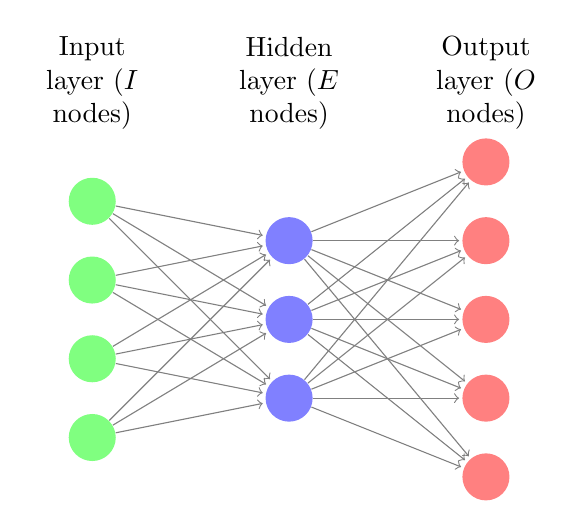
\begin{tikzpicture}[shorten >=1pt,->,draw=black!50, node distance=\layersep]
    \tikzstyle{every pin edge}=[<-,shorten <=1pt]
    \tikzstyle{neuron}=[circle,fill=black!25,minimum size=17pt,inner sep=0pt]
    \tikzstyle{input neuron}=[neuron, fill=green!50];
    \tikzstyle{output neuron}=[neuron, fill=red!50];
    \tikzstyle{hidden neuron}=[neuron, fill=blue!50];
    \tikzstyle{annot} = [text width=4em, text centered]

    \node[input neuron] (I-1) at (0, -1) {};
    \node[input neuron] (I-2) at (0, -2) {};
    \node[input neuron] (I-3) at (0, -3) {};
    \node[input neuron] (I-4) at (0, -4) {};

    \node[hidden neuron] (H-1) at (\layersep, -1.5) {};
    \node[hidden neuron] (H-2) at (\layersep, -2.5) {};
    \node[hidden neuron] (H-3) at (\layersep, -3.5) {};

    \node[output neuron] (O-1) at (\layersep * 2, -0.5) {};
    \node[output neuron] (O-2) at (\layersep * 2, -1.5) {};
    \node[output neuron] (O-3) at (\layersep * 2, -2.5) {};
    \node[output neuron] (O-4) at (\layersep * 2, -3.5) {};
    \node[output neuron] (O-5) at (\layersep * 2, -4.5) {};

    % Connect every node in the input layer with every node in the
    % hidden layer.
    \foreach \source in {1,...,4}
        \foreach \dest in {1,...,3}
            \path (I-\source) edge (H-\dest);

    % Connect every node in the hidden layer with the output layer
    \foreach \source in {1,...,3}
      \foreach \dest in {1,...,5}
        \path (H-\source) edge (O-\dest);

    % Annotate the layers
    \node[annot,above of=H-1, node distance=2cm] (hl) {Hidden layer ($E$ nodes)};
    \node[annot,left of=hl] {Input layer ($I$ nodes)};
    \node[annot,right of=hl] {Output layer ($O$ nodes)};

\end{tikzpicture}